\documentclass[10pt]{article}

\usepackage[a4paper,margin=0.65in]{geometry}
\usepackage{amsmath,amssymb}
\usepackage{graphicx}
\usepackage{booktabs}
\usepackage{array}
\usepackage{float}
\usepackage{hyperref}
\usepackage{enumitem}
\usepackage{xcolor}
\usepackage{tikz}
\usetikzlibrary{positioning,arrows.meta,shapes.geometric}

\setlist{nosep,leftmargin=*}
\renewcommand{\arraystretch}{1.2}
\setlength{\parindent}{0pt}
\setlength{\parskip}{2pt}

\tikzset{
layer/.style={
draw,
rounded corners,
minimum width=1.5cm,
minimum height=0.6cm,
align=center,
fill=blue!10,
font=\scriptsize
},
arrow/.style={
-{Latex[length=2mm]},
thin
}
}

\begin{document}

%%%%%%%%%%%%%%%%%%%%%%%%%%%%%%%%%%%%%%%%%%%%%%%%%%%%%%%%%%%%
% TITLE
%%%%%%%%%%%%%%%%%%%%%%%%%%%%%%%%%%%%%%%%%%%%%%%%%%%%%%%%%%%%

\begin{center}

{\large\textbf{Shiv Nadar University Chennai}}

\vspace{2mm}

{\normalsize\textbf{CS3807 -- Deep Learning Laboratory}}

\vspace{2mm}

{\large\textbf{Experiment 5}}

\vspace{1mm}

{\normalsize\textbf{Comprehensive Study of CNN Training, Regularization,}}

{\normalsize\textbf{Optimization, Hyperparameter Tuning, Transfer Learning}}

{\normalsize\textbf{and Cross-Validation}}

\end{center}

\vspace{3mm}

\begin{tabular}{|p{3.4cm}|p{9.0cm}|p{1.4cm}|}
\hline
Degree \& Branch &
B.Tech Artificial Intelligence \& Data Science &
Semester V\\
\hline
Subject Code \& Name &
CS3807 -- Deep Learning Laboratory &
AY: 2026--27\\
\hline
\end{tabular}

%%%%%%%%%%%%%%%%%%%%%%%%%%%%%%%%%%%%%%%%%%%%%%%%%%%%%%%%%%%%
\section*{1. Objective}

The objective of this experiment is to systematically study the effect of
weight initialization, regularization, optimization algorithms, CNN
hyperparameters, transfer learning, fine-tuning and cross-validation on
image classification performance.

The experiment uses a single CNN architecture, MobileNetV2, and the
Oxford-IIIT Pet dataset. Students will analyze the effect of individual
design choices using training/validation curves and finally select a
suitable configuration using 5-fold cross-validation.

%%%%%%%%%%%%%%%%%%%%%%%%%%%%%%%%%%%%%%%%%%%%%%%%%%%%%%%%%%%%
\section*{2. Learning Outcomes}

After completing this experiment, students will be able to:

\begin{itemize}
\item explain different weight initialization strategies;
\item identify and analyze overfitting using training and validation curves;
\item compare SGD, Momentum, RMSProp and Adam;
\item explain CNN hyperparameters such as kernel size, stride, padding and pooling;
\item understand Batch Normalization and Dropout;
\item perform transfer learning and fine-tuning using MobileNetV2;
\item tune important training hyperparameters;
\item apply 5-fold cross-validation for model selection; and
\item justify the final model using accuracy, variability and computational cost.
\end{itemize}

%%%%%%%%%%%%%%%%%%%%%%%%%%%%%%%%%%%%%%%%%%%%%%%%%%%%%%%%%%%%
\section*{3. Dataset and Experimental Setup}

\textbf{Dataset: Oxford-IIIT Pet Dataset}

The Oxford-IIIT Pet Dataset contains images of cats and dogs belonging
to 37 breeds. The images are RGB and have different spatial dimensions.
For this experiment, all images are resized to

\[
224\times224\times3.
\]

The dataset is suitable for demonstrating transfer learning using
ImageNet-pretrained CNNs.

\textbf{Experimental considerations:}

\begin{itemize}
\item Use RGB images resized to $224\times224$.
\item Normalize the input images according to the pretrained model requirements.
\item Maintain separate training, validation and test data.
\item The test set must remain untouched during hyperparameter selection.
\item Use MobileNetV2 because it is computationally lighter than many
large CNN architectures and is more suitable for CPU-based laboratory work.
\end{itemize}

%%%%%%%%%%%%%%%%%%%%%%%%%%%%%%%%%%%%%%%%%%%%%%%%%%%%%%%%%%%%
\section*{4. MobileNetV2 Architecture}

MobileNetV2 is a lightweight CNN architecture designed to reduce
computational complexity while maintaining good image representation.

Its important components include:

\begin{itemize}
\item depthwise convolution;
\item pointwise $1\times1$ convolution;
\item inverted residual blocks;
\item linear bottlenecks;
\item batch normalization; and
\item ReLU6 activation.
\end{itemize}

A simplified representation is:

\begin{center}
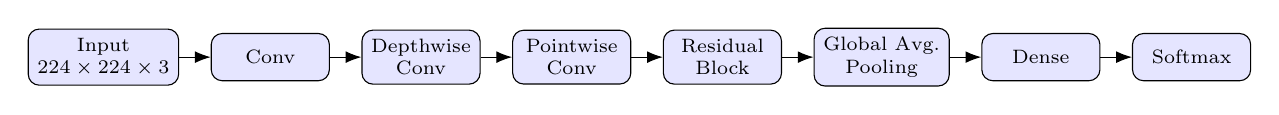
\begin{tikzpicture}[node distance=4mm]

\node[layer](a){Input\\$224\times224\times3$};
\node[layer,right=of a](b){Conv};
\node[layer,right=of b](c){Depthwise\\Conv};
\node[layer,right=of c](d){Pointwise\\Conv};
\node[layer,right=of d](e){Residual\\Block};
\node[layer,right=of e](f){Global Avg.\\Pooling};
\node[layer,right=of f](g){Dense};
\node[layer,right=of g](h){Softmax};

\foreach \x/\y in {a/b,b/c,c/d,d/e,e/f,f/g,g/h}
\draw[arrow](\x)--(\y);

\end{tikzpicture}
\end{center}

\textbf{Note:} The above diagram is a simplified conceptual representation
rather than the complete MobileNetV2 architecture.

%%%%%%%%%%%%%%%%%%%%%%%%%%%%%%%%%%%%%%%%%%%%%%%%%%%%%%%%%%%%
\section*{5. Weight Initialization}

Weight initialization determines the initial values of trainable weights
before training begins. A suitable initialization can improve convergence
and reduce problems such as vanishing or exploding activations.

Students should investigate:

\begin{itemize}
\item Zero initialization
\item Random initialization
\item Xavier/Glorot initialization
\item He initialization
\end{itemize}

\subsection*{Expected Analysis}

Students should compare the initialization strategies using:

\textbf{Plot 1: Training Loss vs. Epoch}

\begin{itemize}
\item X-axis: Epoch
\item Y-axis: Training Loss
\item Plot one curve for each initialization method.
\end{itemize}

\textbf{Plot 2: Validation Accuracy vs. Epoch}

\begin{itemize}
\item X-axis: Epoch
\item Y-axis: Validation Accuracy (\%)
\item Plot one curve for each initialization method.
\end{itemize}

Students should identify which initialization gives faster and more
stable convergence.

%%%%%%%%%%%%%%%%%%%%%%%%%%%%%%%%%%%%%%%%%%%%%%%%%%%%%%%%%%%%
\section*{6. Regularization and Overfitting}

Overfitting occurs when a model performs very well on the training data
but generalizes poorly to unseen data.

Students should compare:

\begin{itemize}
\item No regularization
\item L2 regularization
\item Dropout
\item Batch Normalization
\end{itemize}

\subsection*{Expected Plots}

\textbf{Plot 3: Training and Validation Accuracy vs. Epoch}

\begin{itemize}
\item X-axis: Epoch
\item Y-axis: Accuracy (\%)
\item Plot separate curves for training and validation accuracy.
\end{itemize}

Students should identify the generalization gap.

\textbf{Plot 4: Training and Validation Loss vs. Epoch}

\begin{itemize}
\item X-axis: Epoch
\item Y-axis: Loss
\item Plot training and validation loss.
\end{itemize}

Students should identify whether validation loss begins to increase while
training loss continues to decrease.

%%%%%%%%%%%%%%%%%%%%%%%%%%%%%%%%%%%%%%%%%%%%%%%%%%%%%%%%%%%%
\section*{7. Batch Normalization}

Batch Normalization normalizes activations within a mini-batch during
training.

For a mini-batch

\[
x_1,x_2,\ldots,x_m,
\]

the batch mean is

\[
\mu_B=\frac{1}{m}\sum_{i=1}^{m}x_i
\]

and the batch variance is

\[
\sigma_B^2=
\frac{1}{m}\sum_{i=1}^{m}(x_i-\mu_B)^2.
\]

The normalized activation is

\[
\hat{x}_i=
\frac{x_i-\mu_B}
{\sqrt{\sigma_B^2+\epsilon}}.
\]

The final output is

\[
y_i=\gamma\hat{x}_i+\beta,
\]

where $\gamma$ and $\beta$ are learnable parameters.

\subsection*{Numerical Example}

Consider

\[
x=[2,4,6,8].
\]

The mean is

\[
\mu_B=\frac{2+4+6+8}{4}=5.
\]

The variance is

\[
\sigma_B^2=
\frac{(2-5)^2+(4-5)^2+(6-5)^2+(8-5)^2}{4}
=5.
\]

Therefore,

\[
\sqrt{5}\approx2.236.
\]

Ignoring the very small $\epsilon$,

\[
\hat{x}_1=\frac{2-5}{2.236}\approx-1.342,
\]

\[
\hat{x}_2=\frac{4-5}{2.236}\approx-0.447,
\]

\[
\hat{x}_3=\frac{6-5}{2.236}\approx0.447,
\]

\[
\hat{x}_4=\frac{8-5}{2.236}\approx1.342.
\]

Hence,

\[
\boxed{
\hat{x}\approx[-1.342,-0.447,0.447,1.342]
}
\]

If $\gamma=1$ and $\beta=0$, these are the final outputs.

\textbf{Inference:} Batch Normalization produces approximately
zero-centred and unit-scaled activations for this mini-batch. The
learnable $\gamma$ and $\beta$ allow the network to learn an appropriate
scale and shift.

\textbf{Plot 5: With vs. Without Batch Normalization}

\begin{itemize}
\item X-axis: Epoch
\item Y-axis: Validation Accuracy (\%)
\item Compare two curves: With BN and Without BN.
\end{itemize}

%%%%%%%%%%%%%%%%%%%%%%%%%%%%%%%%%%%%%%%%%%%%%%%%%%%%%%%%%%%%
\section*{8. Optimization Algorithms}

Students should compare the following optimization methods:

\begin{itemize}
\item SGD
\item Momentum
\item RMSProp
\item Adam
\end{itemize}

The objective is to study convergence speed, stability and final
validation performance.

\textbf{Plot 6: Training Loss vs. Epoch for Different Optimizers}

\begin{itemize}
\item X-axis: Epoch
\item Y-axis: Training Loss
\item One curve for each optimizer.
\end{itemize}

\textbf{Plot 7: Validation Accuracy vs. Epoch for Different Optimizers}

\begin{itemize}
\item X-axis: Epoch
\item Y-axis: Validation Accuracy (\%)
\item One curve for each optimizer.
\end{itemize}

\begin{center}
\begin{tabular}{|l|c|c|c|c|}
\hline
Optimizer & Final Loss & Best Val. Accuracy & Epoch to Converge & Time\\
\hline
SGD & & & &\\
Momentum & & & &\\
RMSProp & & & &\\
Adam & & & &\\
\hline
\end{tabular}
\end{center}

%%%%%%%%%%%%%%%%%%%%%%%%%%%%%%%%%%%%%%%%%%%%%%%%%%%%%%%%%%%%
\section*{9. CNN Hyperparameter Tuning}

The following hyperparameters should be investigated:

\begin{center}
\begin{tabular}{|l|l|}
\hline
Hyperparameter & Suggested Values\\
\hline
Learning Rate & $0.001,\;0.0001$\\
Batch Size & 16, 32, 64\\
Dropout Rate & 0, 0.25, 0.5\\
Optimizer & SGD, Adam\\
Fine-Tuning Learning Rate & $10^{-4},10^{-5}$\\
Frozen Layers & Frozen base / Partial unfreezing\\
\hline
\end{tabular}
\end{center}

For CNN concepts, students should also understand:

\begin{itemize}
\item kernel/filter;
\item stride;
\item padding;
\item pooling;
\item number of channels; and
\item depthwise separable convolution.
\end{itemize}

For a convolution operation, the output dimension can be calculated as

\[
O=
\left\lfloor
\frac{N+2P-K}{S}
\right\rfloor+1,
\]

where $N$ is input size, $K$ is kernel size, $P$ is padding and $S$ is
stride.

\textbf{Experimental rule:} During a controlled hyperparameter study,
change one hyperparameter at a time while keeping the remaining settings
fixed.

\textbf{Plot 8: Learning Rate vs. Validation Accuracy}

\begin{itemize}
\item X-axis: Learning Rate
\item Y-axis: Validation Accuracy (\%)
\end{itemize}

\textbf{Plot 9: Batch Size vs. Validation Accuracy}

\begin{itemize}
\item X-axis: Batch Size
\item Y-axis: Validation Accuracy (\%)
\end{itemize}

\textbf{Plot 10: Dropout Rate vs. Validation Accuracy}

\begin{itemize}
\item X-axis: Dropout Rate
\item Y-axis: Validation Accuracy (\%)
\end{itemize}

%%%%%%%%%%%%%%%%%%%%%%%%%%%%%%%%%%%%%%%%%%%%%%%%%%%%%%%%%%%%
\section*{10. Transfer Learning and Fine-Tuning}

MobileNetV2 pretrained on ImageNet should be used.

\subsection*{Case A: Feature Extraction}

\[
\text{Pretrained MobileNetV2}
\rightarrow
\text{Freeze Base}
\rightarrow
\text{New Classifier}
\]

The pretrained convolutional layers are frozen and only the newly added
classification layers are trained.

\subsection*{Case B: Fine-Tuning}

\[
\text{Pretrained MobileNetV2}
\rightarrow
\text{Unfreeze Selected Layers}
\rightarrow
\text{Small Learning Rate}
\]

The upper layers of the pretrained network are unfrozen and trained with
a smaller learning rate.

\textbf{Plot 11: Feature Extraction vs. Fine-Tuning}

\begin{itemize}
\item X-axis: Epoch
\item Y-axis: Validation Accuracy (\%)
\item Two curves: Feature Extraction and Fine-Tuning.
\end{itemize}

\textbf{Plot 12: Training and Validation Loss}

Students should compare the loss curves before and after fine-tuning.

\textbf{Discussion:} Explain why fine-tuning normally requires a smaller
learning rate than training a newly initialized classifier.

%%%%%%%%%%%%%%%%%%%%%%%%%%%%%%%%%%%%%%%%%%%%%%%%%%%%%%%%%%%%
\section*{11. K-Fold Cross-Validation}

After the individual studies, select 3--4 promising configurations.

Use 5-fold cross-validation on the training data.

For $K=5$,

\[
\bar{A}=
\frac{1}{5}\sum_{i=1}^{5}A_i
\]

and

\[
SD=
\sqrt{
\frac{1}{5}
\sum_{i=1}^{5}(A_i-\bar{A})^2
}.
\]

Report the result as

\[
\boxed{\bar{A}\pm SD}.
\]

The independent test set must not be used during hyperparameter selection.

\begin{center}
\begin{tabular}{|l|c|c|c|c|c|c|}
\hline
Configuration & F1 & F2 & F3 & F4 & F5 & Mean $\pm$ SD\\
\hline
C1 & & & & & &\\
C2 & & & & & &\\
C3 & & & & & &\\
C4 & & & & & &\\
\hline
\end{tabular}
\end{center}

\textbf{Plot 13: 5-Fold Cross-Validation Accuracy}

\begin{itemize}
\item X-axis: Hyperparameter Configuration
\item Y-axis: Mean Validation Accuracy (\%)
\item Include standard-deviation error bars.
\end{itemize}

Students should discuss both mean performance and variability.

%%%%%%%%%%%%%%%%%%%%%%%%%%%%%%%%%%%%%%%%%%%%%%%%%%%%%%%%%%%%
\section*{12. Final Model Evaluation}

After selecting the best configuration using cross-validation:

\begin{enumerate}
\item Retrain the selected configuration using the complete training data.
\item Keep the independent test set untouched until this stage.
\item Evaluate the final model on the test set.
\end{enumerate}

Report:

\begin{center}
\begin{tabular}{|l|c|}
\hline
Metric & Value\\
\hline
Mean CV Accuracy &\\
CV Standard Deviation &\\
Test Accuracy &\\
Precision &\\
Recall &\\
F1-score &\\
Training Time &\\
Number of Parameters &\\
\hline
\end{tabular}
\end{center}

\textbf{Plot 14: Confusion Matrix}

Students should identify:

\begin{itemize}
\item the best classified classes;
\item the most frequently confused classes; and
\item possible visual reasons for misclassification.
\end{itemize}

\textbf{Optional Plot 15: Misclassified Images}

Display representative incorrectly classified images and provide a
brief explanation for each.

%%%%%%%%%%%%%%%%%%%%%%%%%%%%%%%%%%%%%%%%%%%%%%%%%%%%%%%%%%%%
\section*{13. Source Code}

The complete source code is attached separately in the GitHub repository and submitted along with this report.

\textbf{GitHub Repository:}

\url{https://github.com/Sadhana2006-art/Deep-Learning-Lab}

\section*{14. Results}

Optimization Algorithms:

\begin{center}
\begin{tabular}{|l|c|c|c|c|}
\hline
Optimizer & Final Loss & Best Val. Accuracy & Epoch to Converge & Time\\
\hline
SGD & 0.1402 & 91.85\% & 10 & 183.04 \\
Momentum & 0.0074 & 92.39\% & 9 & 253.35 \\
RMSProp & 0.0016 & 92.26\% & 9 & 258.68 \\
Adam & 0.0053 & 92.80\% & 10 & 267.21 \\
\hline
\end{tabular}
\end{center}

K-Fold Cross-Validation:

\begin{center}
\begin{tabular}{|l|c|c|c|c|c|c|}
\hline
Configuration & F1 & F2 & F3 & F4 & F5 & Mean $\pm$ SD\\
\hline
C1 & 91.34\% & 90.66\% & 91.68\% & 92.36\% & 92.52\% & 91.71\% $\pm$ 0.68\%\\
C2 & 91.00\% & 92.19\% & 91.51\% & 91.85\% & 92.18\% & 91.75\% $\pm$ 0.45\%\\
C3 & 91.00\% & 91.34\% & 91.68\% & 91.85\% & 92.52\% & 91.68\% $\pm$ 0.51\%\\
C4 & 83.87\% & 84.89\% & 86.42\% & 87.10\% & 88.95\% & 86.24\% $\pm$ 1.76\%\\
\hline
\end{tabular}
\end{center}

Final Model Evaluation:

\begin{center}
\begin{tabular}{|l|c|}
\hline
Metric & Value\\
\hline
Mean CV Accuracy & 91.75\% \\
CV Standard Deviation & 0.45\% \\
Test Accuracy & 89.42\% \\
Precision & 89.79\% \\
Recall & 89.42\% \\
F1-score & 89.37\% \\
Training Time & 162.81 s \\
Number of Parameters & 2,426,725 \\
\hline
\end{tabular}
\end{center}

Overall Results:

\begin{center}
\begin{tabular}{|l|c|c|c|c|}
\hline
Configuration & CV Accuracy & SD & Test Accuracy & Training Time\\
\hline
Baseline & 92.7\% & -- & 92.7\% & 201.47 s\\
Best Initialization (Xavier/Glorot) & 93.1\% & -- & 93.1\% & 254.81 s\\
Best Regularization (Batch Normalization) & 92.3\% & -- & 92.3\% & 211.91 s\\
Best Optimizer (Adam) & 92.7\% & -- & 92.7\% & 267.21 s\\
Best Hyperparameters (C2) & 91.75\% & 0.45\% & 89.42\% & 162.81 s\\
Fine-Tuned Model & 90.22\% & -- & 90.22\% & 259.18 s\\
\hline
\end{tabular}
\end{center}

The configuration C2 was chosen because it had the best average 5 fold cross-validation accuracy at 91.75\%, and it also had the least standard deviation at 0.45\%. This means that it was not only an accurate configuration, but also it produced similar results across all folds, thus consistency of results. C2 took the least time to train at 162.81 seconds among the other main configurations. After re-training on the full training set, C2 gave an independent test accuracy of 89.42\% with Precision, Recall and F1-score being 89.79\%, 89.42\% and 89.37\%, respectively.

%%%%%%%%%%%%%%%%%%%%%%%%%%%%%%%%%%%%%%%%%%%%%%%%%%%%%%%%%%%%
\section*{15. Plots with Inference}

\subsection*{15.1 Training Loss vs Epoch for Different Weight Initializations}

\begin{figure}[H]
\centering

\includegraphics[width=\textwidth]{Training_Loss_vs_Epoch.eps}
\caption{Training Loss vs Epoch}
\end{figure}

\textbf{Interpretation:}

The initialization curve for the zero initializer remains relatively constant at 3.61, while that of random, Xavier/Glorot, and He goes down to zero very quickly.
The zero initializer fails to provide a good learning process because all neurons have equal weights, hence keeping the training loss constant. The random, Xavier/Glorot, and He initializers break symmetry and enable quick minimization of the training loss.

\subsection*{15.2 Validation Accuracy vs Epoch for Different Weight Initializations}

\begin{figure}[H]
\centering

\includegraphics[width=\textwidth]{Validation_Accuracy_vs_Epoch.eps}
\caption{Validation Accuracy vs Epoch}
\end{figure}

\textbf{Interpretation:}

Zero initialization stays at about 1.9\%, which is close to the chance rate of 37 classes. The other three initialization methods quickly get around 90-93\% validation accuracy.
Zero initialization is unable to learn meaningful class representations and therefore gets nearly the chance-level validation accuracy. Random, Xavier/Glorot, and He initialization successfully break the symmetry, and Xavier/Glorot reaches the best final validation accuracy of approximately 93.1\%.

\subsection*{15.3 Training and Validation Accuracy vs. Epoch}

\begin{figure}[H]
\centering
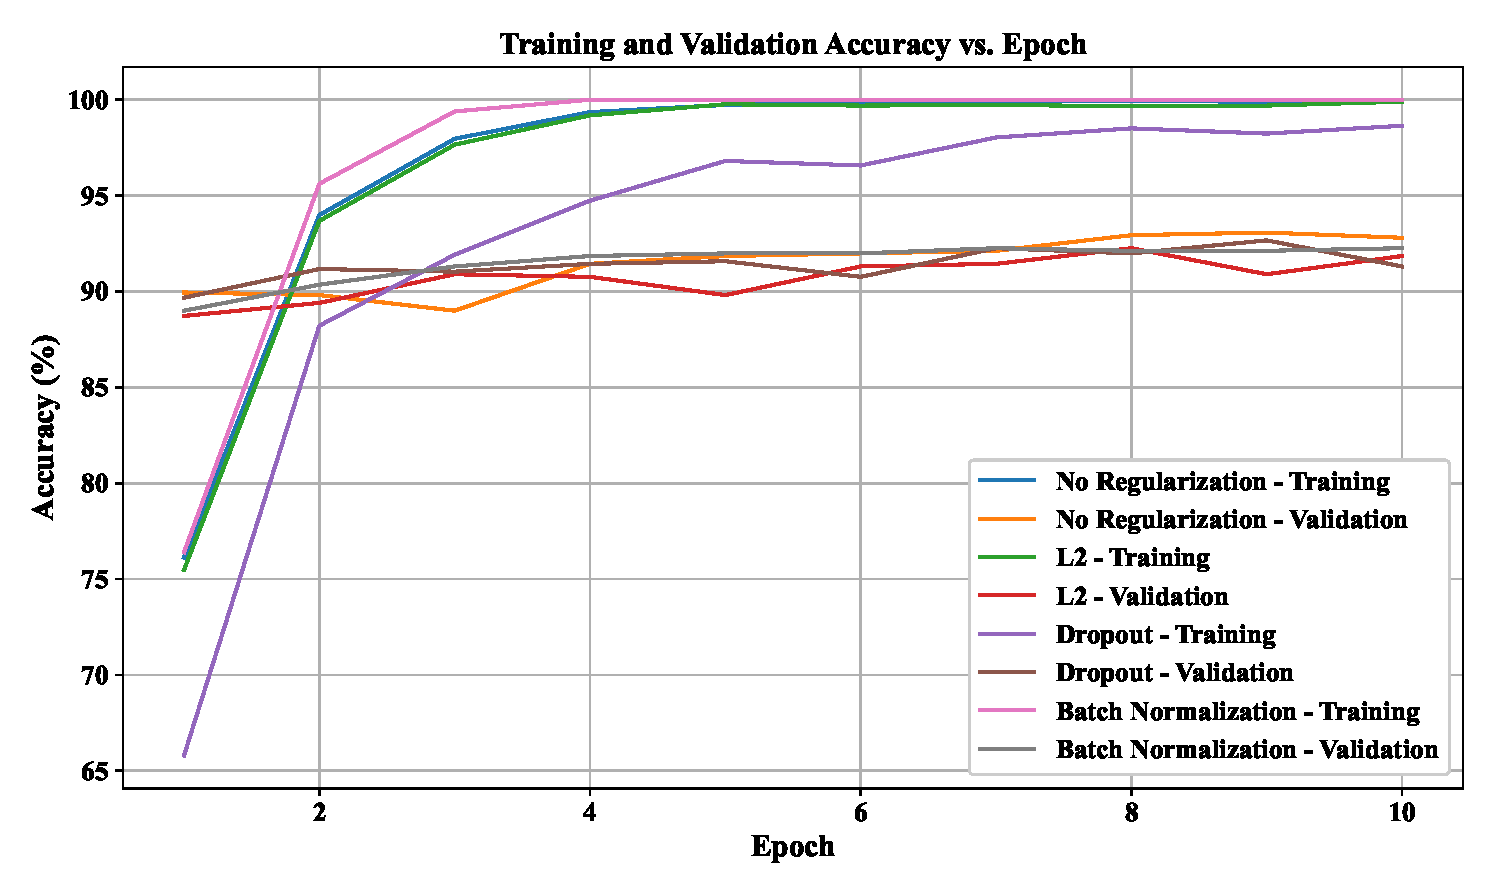
\includegraphics[width=\textwidth]{Training_and_Validation_Accuracy_vs_Epoch.eps}
\caption{Training and Validation Accuracy vs Epoch}
\end{figure}

\textbf{Interpretation:}

The critical thing to note is the generalization gap:

Without Regularization: The training accuracy is nearly 100\%, but the validation remains at 93\%.
With L2: Training accuracy is around 99.9\%, and validation accuracy is about 92.5\%.
With Dropout: Training accuracy is nearly 98.6\%, but validation accuracy is 91.3\%.
With Batch Normalization: Training accuracy is 100\%, and validation accuracy is 92.3\%.
This shows a clear gap between training and validation accuracy, indicating some degree of overfitting.

\subsection*{15.4 Training and Validation Loss vs. Epoch}

\begin{figure}[H]
\centering
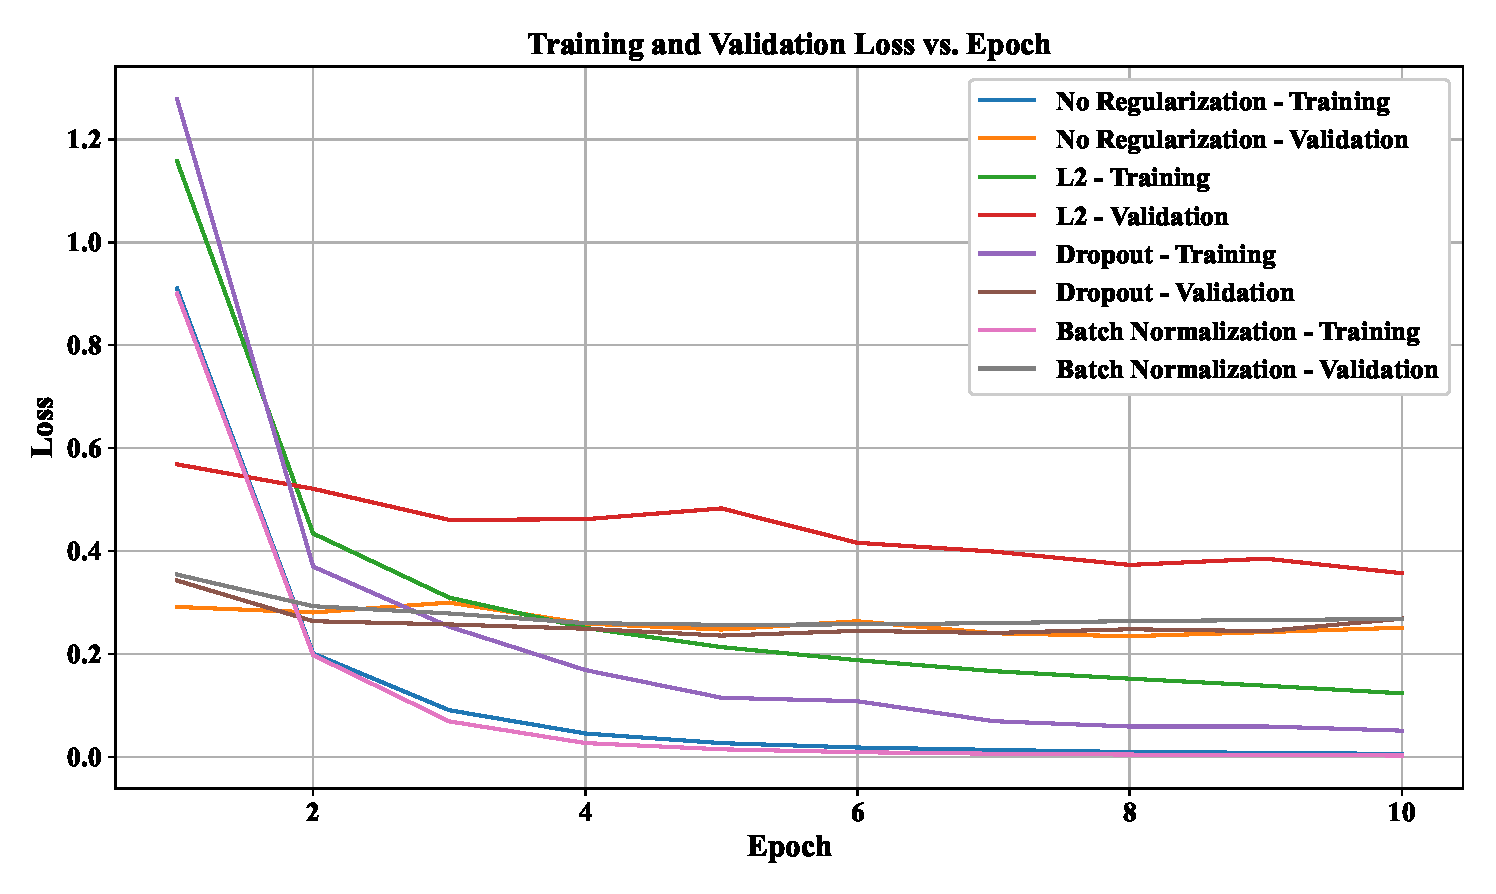
\includegraphics[width=\textwidth]{Training_and_Validation_Loss_vs_Epoch.eps}
\caption{Training and Validation Loss vs Epoch}
\end{figure}

\textbf{Interpretation:}

Yes, that is what happens in Batch Normalization:
Loss during training keeps reducing from approximately 0.90 → 0.003
Loss during validation reduces up to approximately 0.236 at epoch 5
After this, loss during validation begins to increase/fluctuate:
Epoch 6: ~0.258
Epoch 7: ~0.260
Epoch 8: ~0.264
Epoch 9: ~0.266
This is an indication of overfitting.

\subsection*{15.5 Validation Accuracy With vs. Without Batch Normalization}

\begin{figure}[H]
\centering
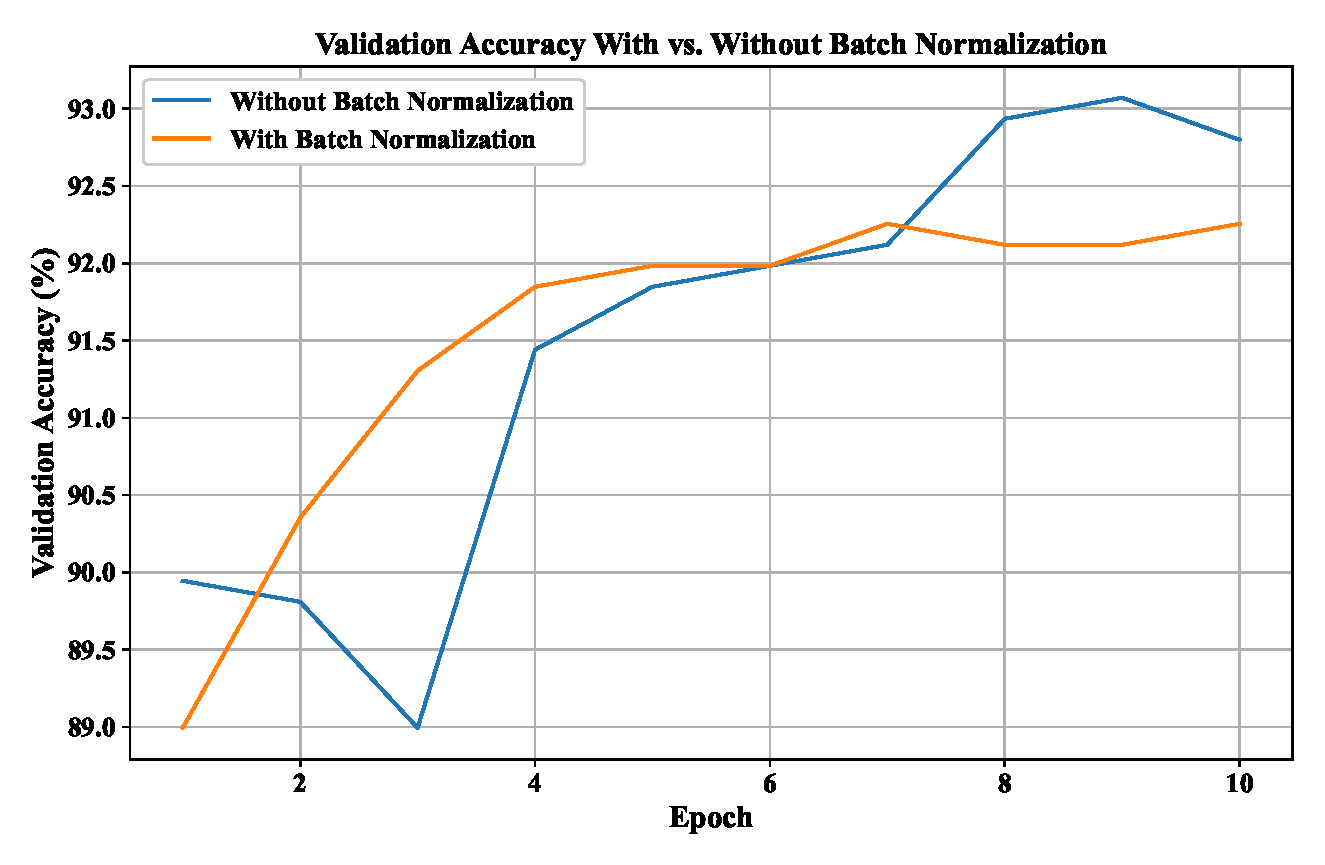
\includegraphics[width=\textwidth]{Batch_Normalization_Comparison.eps}
\caption{Validation Accuracy With vs. Without Batch Normalization}
\end{figure}

\textbf{Interpretation:}

However, batch normalization causes faster increases in validation accuracy in the early epochs. The model that uses batch normalization achieves 92\% accuracy in validation faster than the model without batch normalization. Nevertheless, in about epoch 7, the model without batch normalization overtakes the model with batch normalization by achieving the maximum validation accuracy of about 93.1\%. Therefore, batch normalization helps to learn fast and consistently, but it does not guarantee higher validation accuracy at the end of learning.

\subsection*{15.6 Training Loss vs. Epoch for Different Optimizers}

\begin{figure}[H]
\centering
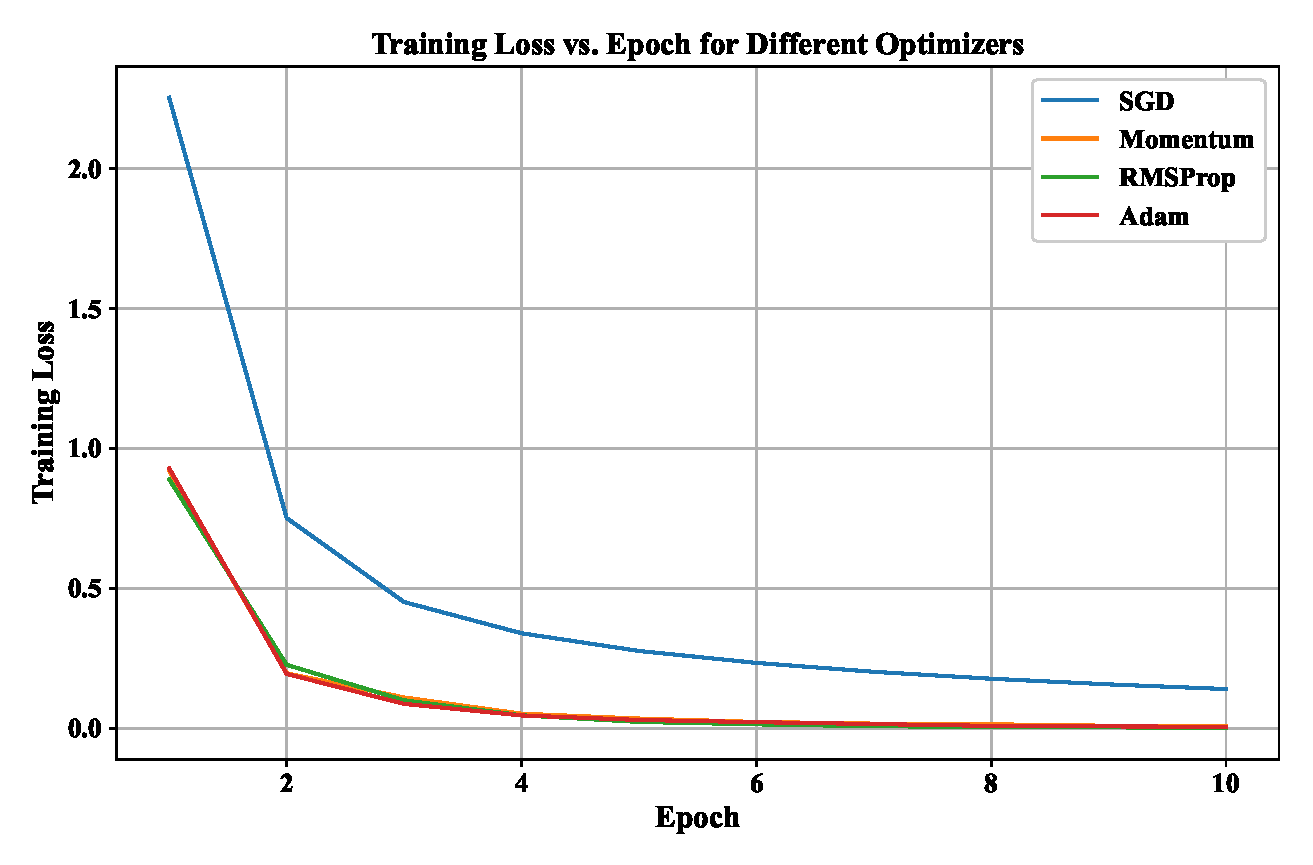
\includegraphics[width=\textwidth]{Optimizer_Training_Loss.eps}
\caption{Training Loss vs Epoch for Different Optimizers}
\end{figure}

\textbf{Interpretation:}

Training loss of the optimizers like SGD, Momentum, RMSProp, and Adam is plotted in the graph. Training loss reduces for all optimizers; however, in the case of RMSProp and Adam, the loss decreases much rapidly compared to the SGD. The adaptive gradient descent is much better than simple SGD.

\subsection*{15.7 Validation Accuracy vs. Epoch for Different Optimizers}

\begin{figure}[H]
\centering
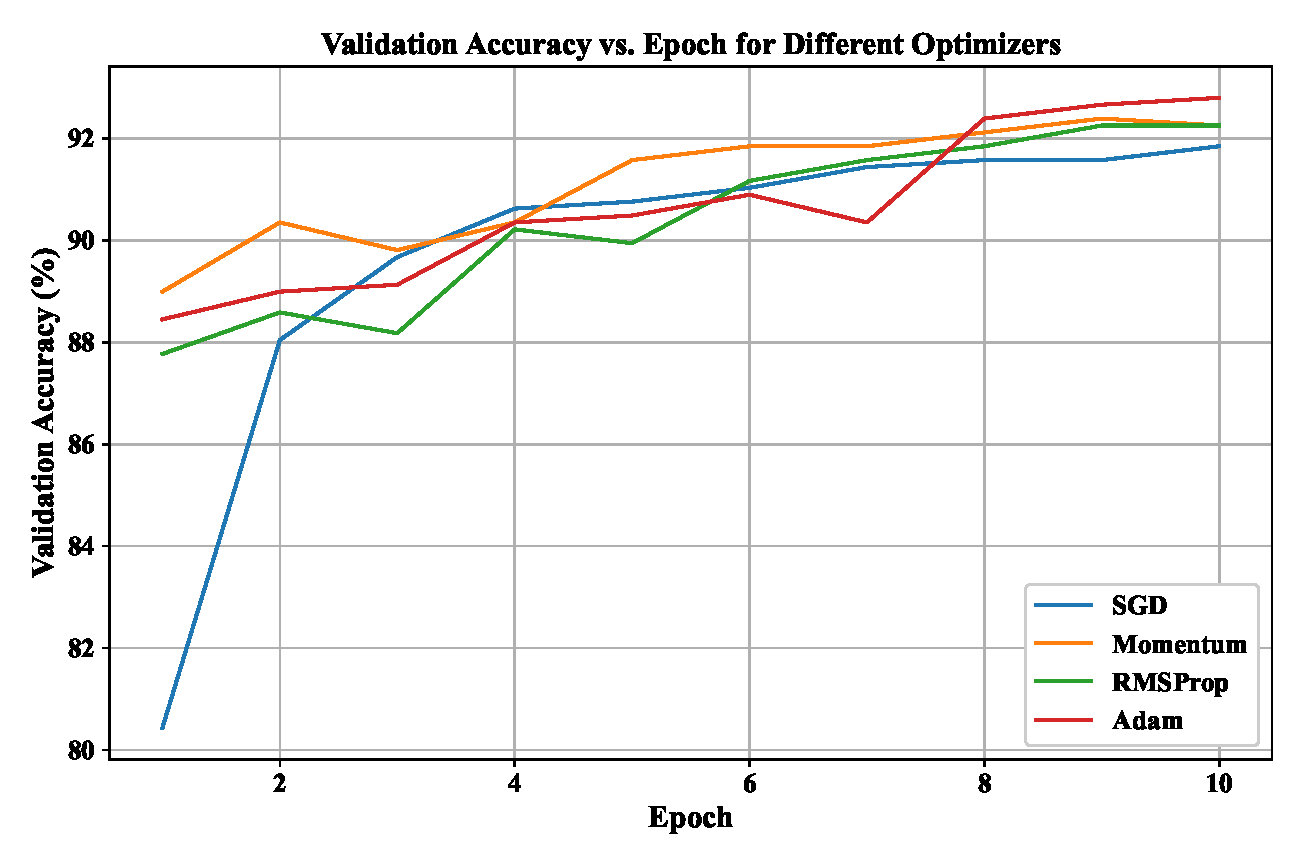
\includegraphics[width=0.75\textwidth]{Optimizer_Validation_Accuracy.eps}
\caption{Validation Accuracy vs Epoch for Different Optimizers}
\end{figure}

\textbf{Interpretation:}

The figure depicts the comparison of validation accuracy among the four optimization methods. Adam exhibits the best performance with 92.8\% validation accuracy, followed by Momentum and RMSProp, whereas SGD gets up to 91.8\%. This difference arises due to the use of different techniques for updating the parameters.

\subsection*{15.8 Learning Rate vs. Validation Accuracy}

\begin{figure}[H]
\centering
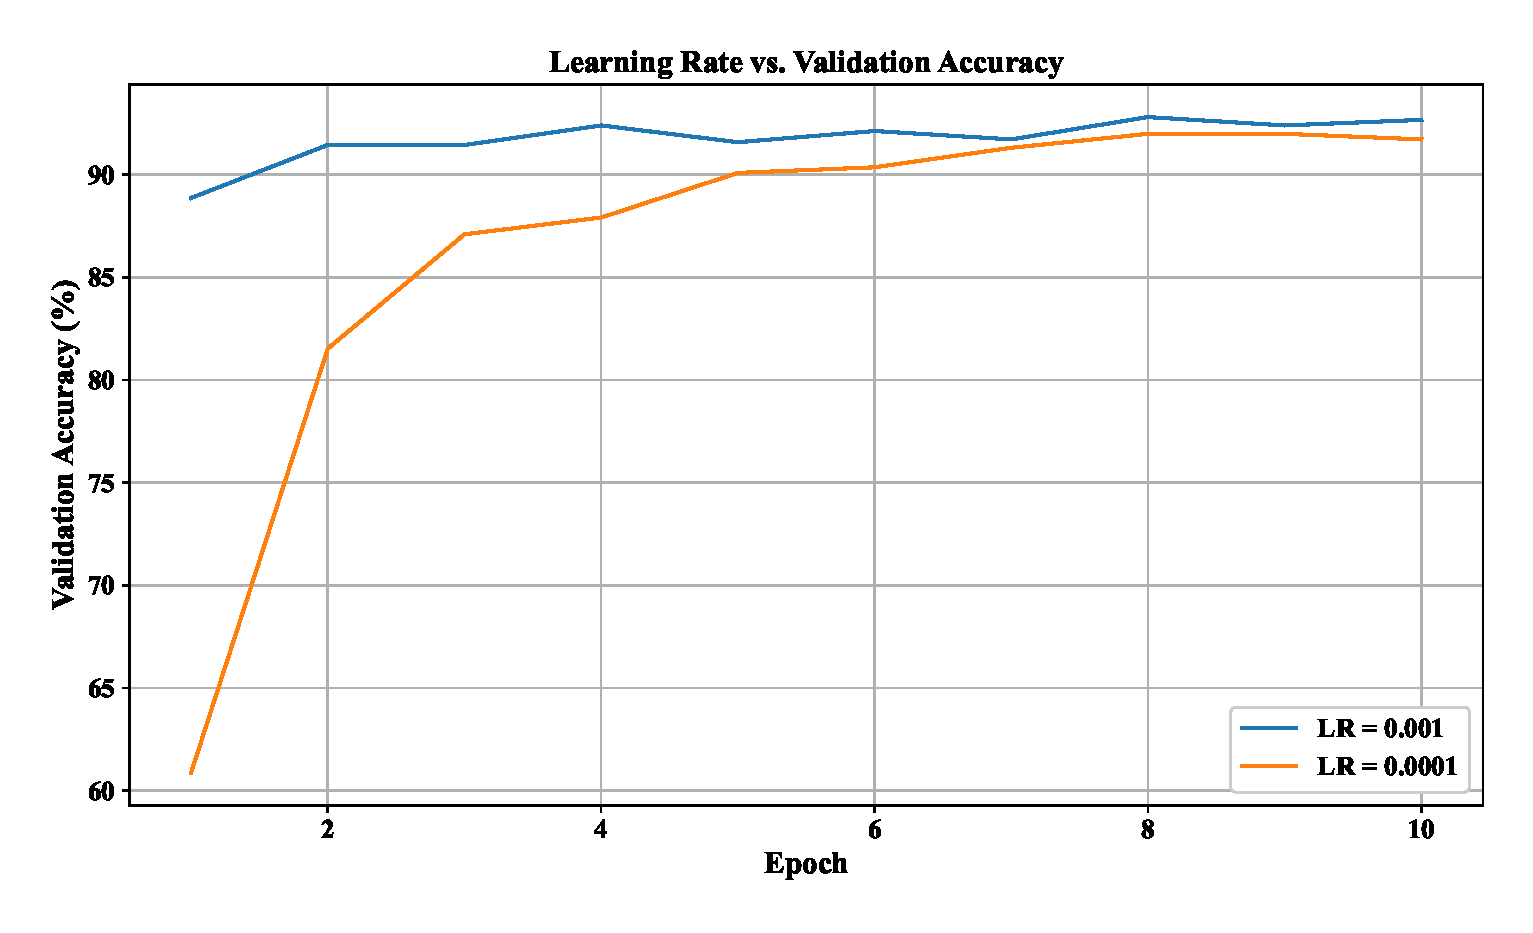
\includegraphics[width=0.75\textwidth]{Learning_Rate_vs_Validation_Accuracy.eps}
\caption{Learning Rate vs. Validation Accuracy}
\end{figure}

\textbf{Interpretation:}

The plot shows the comparison of validation accuracies of learning rates 0.001 and 0.0001. The learning rate of 0.001 gives better validation accuracy compared to that of 0.0001 (validation accuracy of ~92.8\% versus ~91.7\%, respectively). The reason for this could be that 0.001 gives a more efficient update to parameters in limited training epochs.

\subsection*{15.9 Batch Size vs. Validation Accuracy}

\begin{figure}[H]
\centering
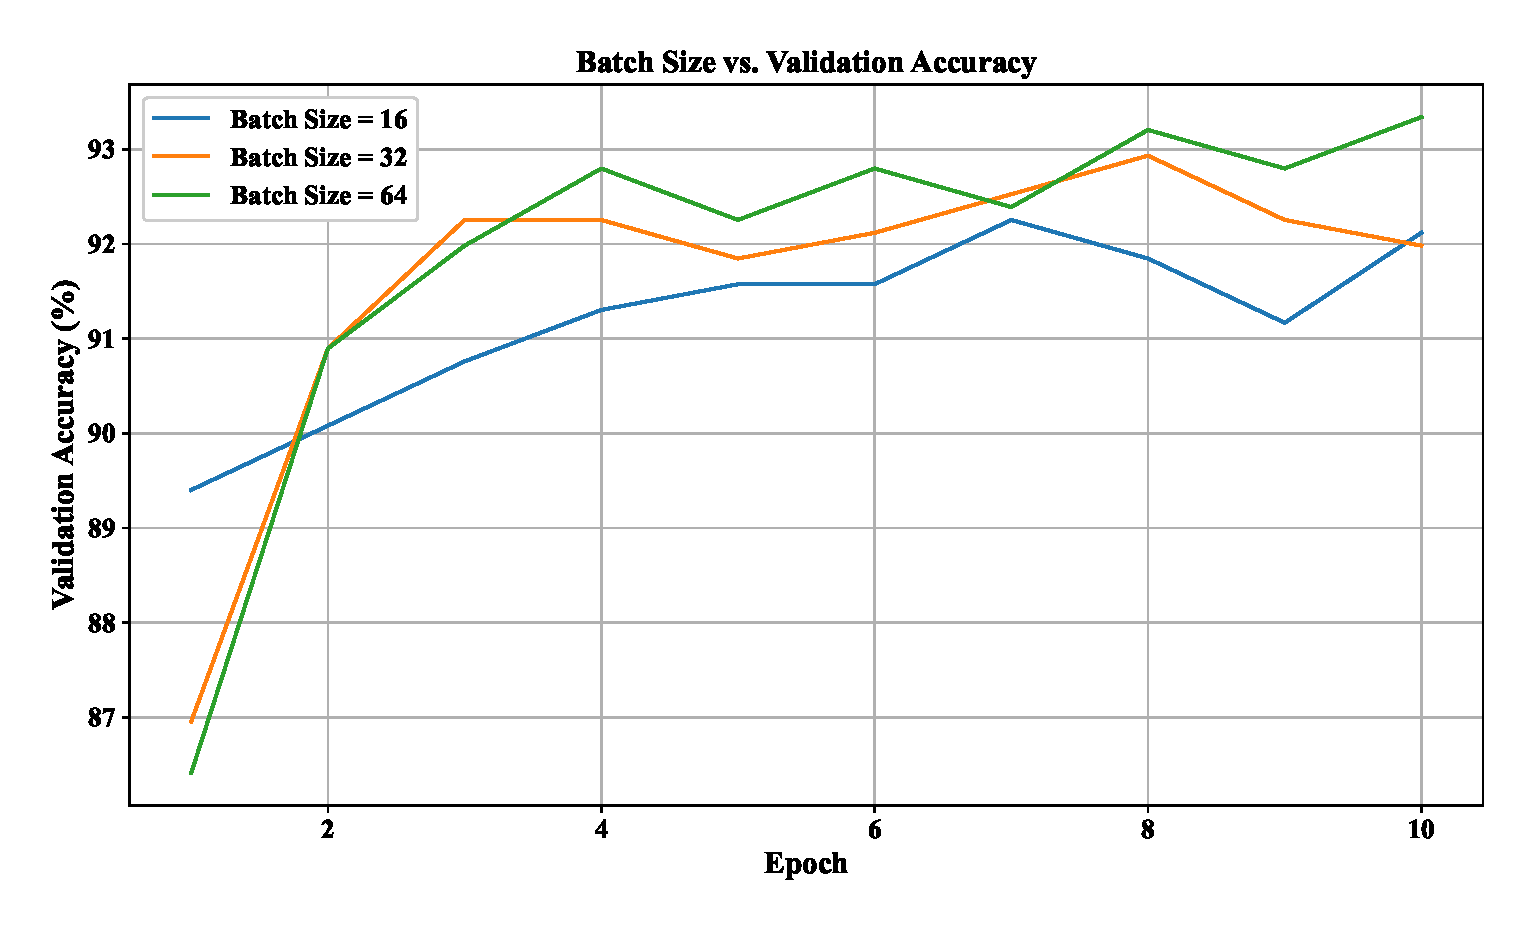
\includegraphics[width=0.75\textwidth]{Batch_Size_vs_Validation_Accuracy.eps}
\caption{Batch Size vs. Validation Accuracy}
\end{figure}

\textbf{Interpretation:}

The graph illustrates the accuracy of validation using different batch sizes such as 16, 32, and 64. The batch size of 64 has attained the highest validation accuracy at around 93.3\% compared to the other sizes. The bigger batch size makes the gradient estimation process more stable.

\subsection*{15.10 Dropout Rate vs. Validation Accuracy}

\begin{figure}[H]
\centering
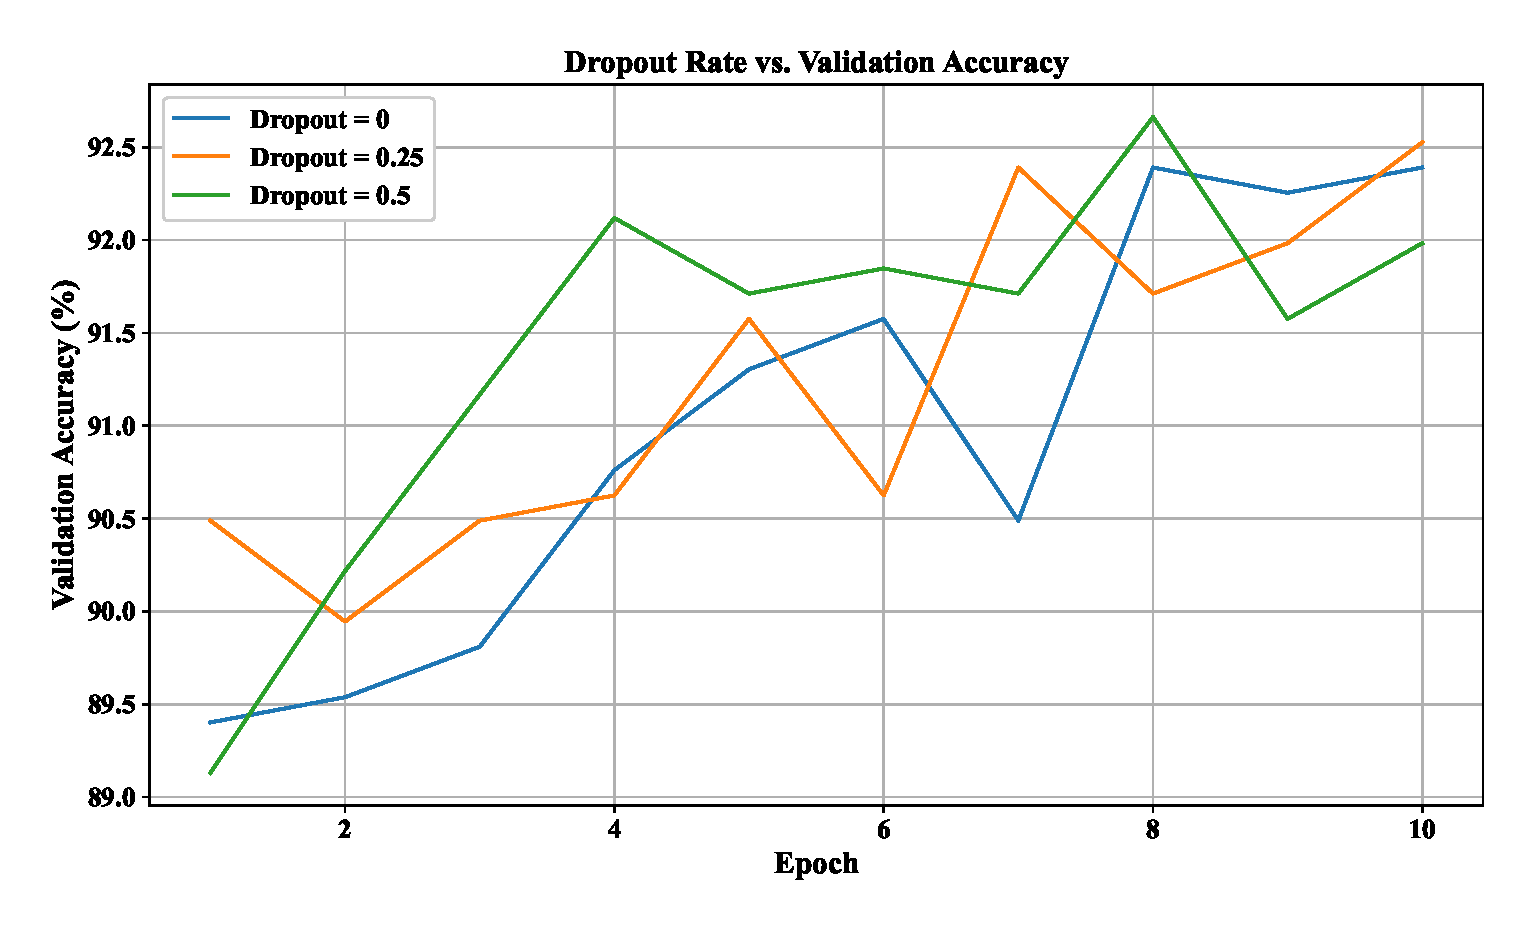
\includegraphics[width=0.75\textwidth]{Dropout_Rate_vs_Validation_Accuracy.eps}
\caption{Dropout Rate vs. Validation Accuracy}
\end{figure}

\textbf{Interpretation:}

The plot illustrates the validation accuracy in relation to the following dropout values: 0, 0.25 and 0.5. For a dropout value of 0.5, there is the highest validation accuracy achieved (~92.7\%). The increased regularization may help in avoiding overfitting through limiting the reliance on specific neurons.

\subsection*{15.11 Feature Extraction vs. Fine-Tuning}

\begin{figure}[H]
\centering
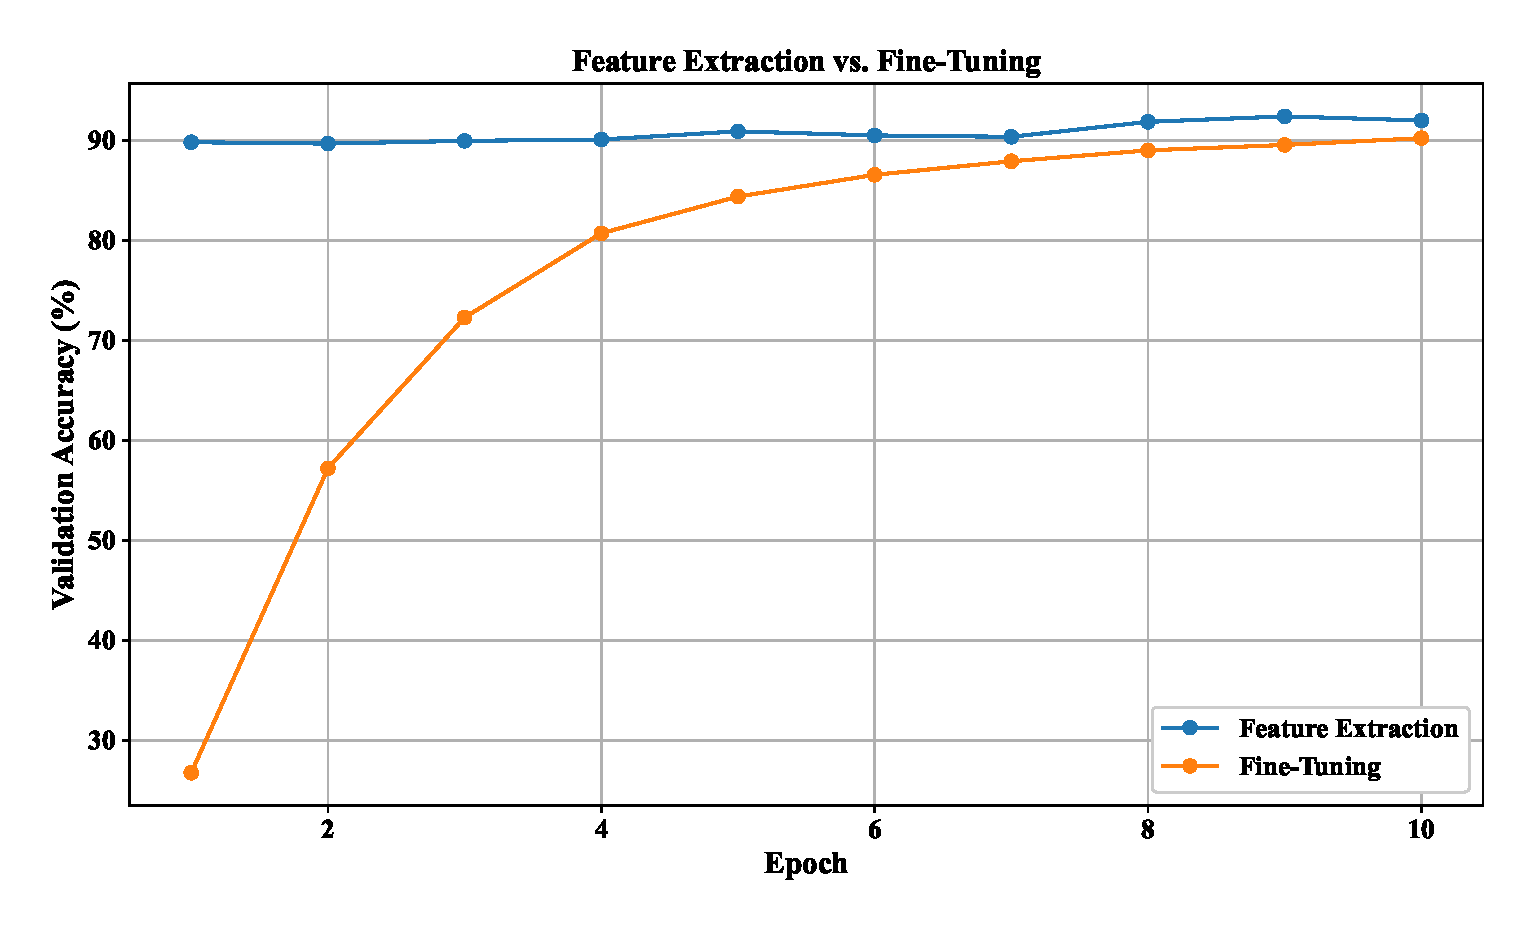
\includegraphics[width=0.75\textwidth]{Feature_Extraction_vs_Fine_Tuning.eps}
\caption{Feature Extraction vs. Fine-Tuning}
\end{figure}

\textbf{Interpretation:}

Validation accuracy performance of feature extraction vs fine-tuning is represented on the graph for 10 epochs. While validation accuracy of feature extraction remains high at 90-92\%, fine-tuning achieves an increase in accuracy from 26.77\% to 90.22\%. Validation accuracy of fine-tuning begins low because the chosen pre-trained layers need to be trained with a small learning rate.

\subsection*{15.12 Training and Validation Loss: Feature Extraction vs. Fine-Tuning}

\begin{figure}[H]
\centering
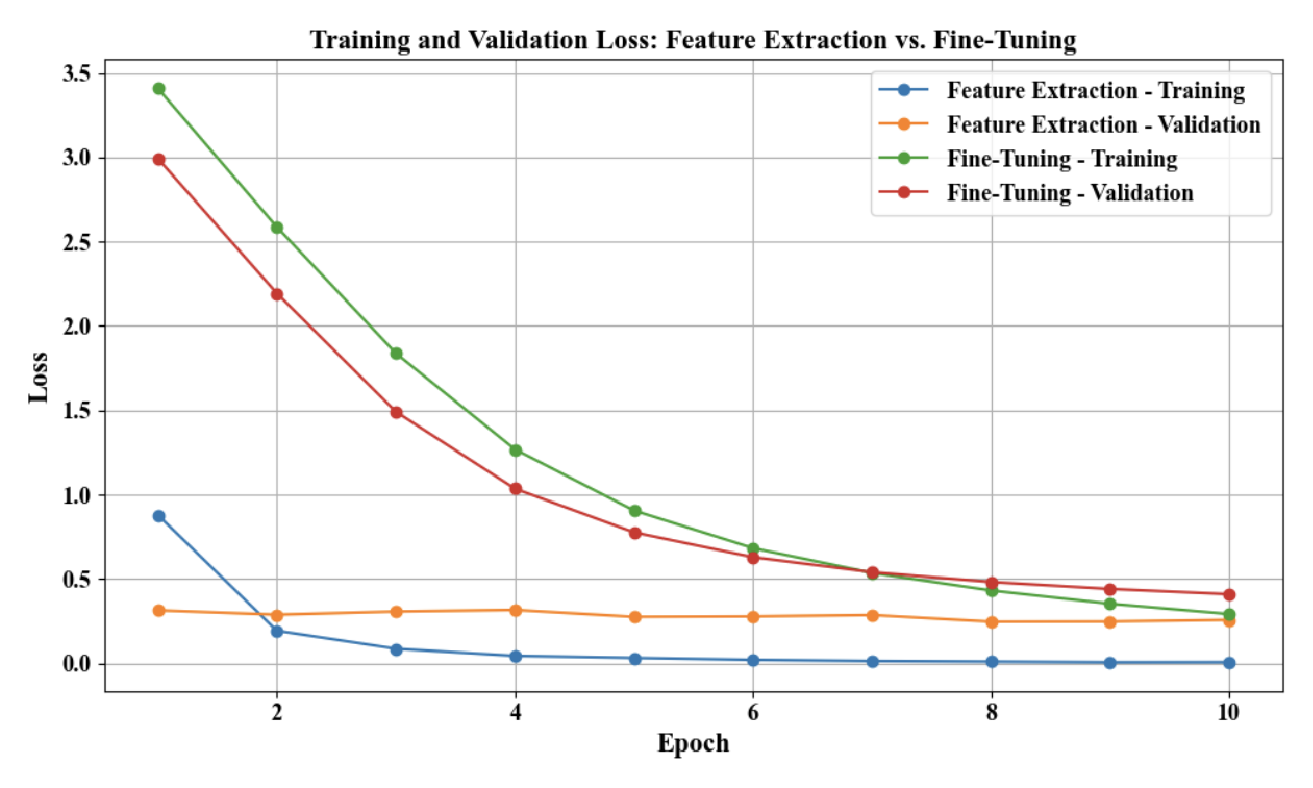
\includegraphics[width=0.75\textwidth]{Training_and_Validation_Loss_Feature_Extraction_vs_Fine_Tuning.eps}
\caption{Training and Validation Loss: Feature Extraction vs. Fine-Tuning}
\end{figure}

\textbf{Interpretation:}

Losses for training and validation have been compared for the model with and without fine-tuning. The loss obtained from feature extraction is significantly lower with 0.0067 for training and 0.2570 for validation; on the other hand, for fine-tuning, loss reduces to 0.2916 for training and 0.4096 for validation. It can be seen that feature extraction works better in a span of 10 epochs.

\subsection*{15.13 5-Fold Cross-Validation Accuracy}

\begin{figure}[H]
\centering
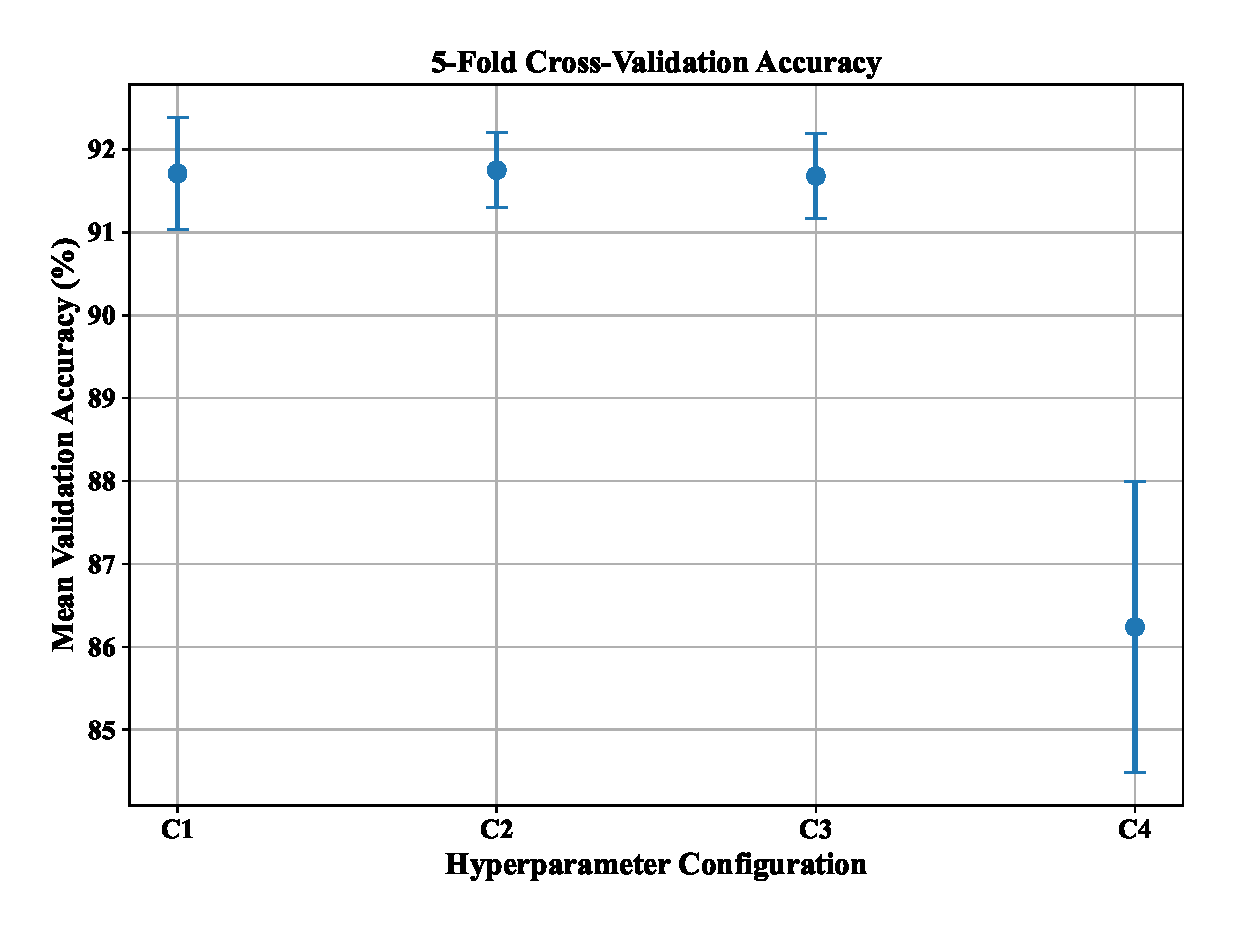
\includegraphics[width=0.75\textwidth]{cv_accuracy.eps}
\caption{5-Fold Cross-Validation Accuracy}
\end{figure}

\textbf{Interpretation:}

In the plot, the validation accuracy means and standard deviations of the four hyperparameter settings are compared using five folds. C1, C2, and C3 have a similar level of accuracy of approximately 91.7\%. C2 is the best in terms of the accuracy mean value (91.75\%) and low variability (±0.45\%).

\subsection*{15.14 Confusion Matrix}

\begin{figure}[H]
\centering
\includegraphics[width=0.75\textwidth]{confusion_matrix.eps}
\caption{Confusion Matrix}
\end{figure}

\textbf{Interpretation:}

From the confusion matrix it is clear that most of the predictions have come along the diagonal path. This implies that the prediction has performed well over all the 37 classes. Misclassification is only seen in case of classes which look alike, i.e. dog breeds like American Pit Bull Terrier and Staffordshire Bull Terrier and cat breeds which also look alike.

\subsection*{15.15 Misclassified Images}

\begin{figure}[H]
\centering
\includegraphics[width=0.75\textwidth]{misclassified_images.eps}
\caption{Misclassified Images}
\end{figure}

\textbf{Interpretation:}

Plot showcases examples of misclassified images and suggests that misclassification mostly happens among those dog and cat breeds that look alike. For instance, Beagle is classified as American Pit Bull Terrier, and Egyptian Mau is classified as Bengal due to some visual resemblance.

%%%%%%%%%%%%%%%%%%%%%%%%%%%%%%%%%%%%%%%%%%%%%%%%%%%%%%%%%%%%
\section*{16. Discussion Questions}

\begin{enumerate}

\item \textbf{What is the difference between model parameters and hyperparameters?}

Model Parameters refer to the automatically acquired value during model training process, for example, weights and biases. Hyperparameters refer to values chosen before the training process begins, like learning rate, batch size, dropout rate, etc.

\item \textbf{Why is weight initialization important?}

Weight Initialization refers to the process of selecting the initial values of the weights of the neural networks. Weight initialization should help the neural network to learn faster and avoid issues like vanishing gradient and symmetric neurons.

\item \textbf{Why can zero initialization be problematic for neural networks?}

Since the initial values of all the weights are set to zero, all neurons learn the same feature since they have the same gradient. This makes it impossible for neurons to learn different representations.

\item \textbf{Compare Xavier and He initialization.}

Xavier initialization is applicable mostly for sigmoid and tanh activation functions and maintains the right level of activation variance. He initialization technique is applicable mostly for ReLU-based networks and is usually more effective for ReLU activations.

\item \textbf{How can training and validation curves be used to identify overfitting?}

In case training accuracy keeps increasing while validation accuracy starts decreasing or remains stagnant, there may be an issue of overfitting. Moreover, in case training loss continues decreasing and validation loss starts increasing, the model is also fitting itself into training data excessively.

\item \textbf{How does Dropout reduce overfitting?}

Dropout technique randomly switches off a certain portion of neurons while training. This helps the neural network not to be overly dependent on specific neurons.

\item \textbf{What is the purpose of Batch Normalization?}

Normalization within a mini-batch is known as Batch Normalization. It enables stabilization and accelerates the training process.

\item \textbf{Explain the numerical Batch Normalization example.}

For $x=[2,4,6,8]$, the batch mean is

\[
\mu_B=5
\]

and the batch variance is

\[
\sigma_B^2=5.
\]

Therefore, the normalized values are approximately

\[
\hat{x}=[-1.342,-0.447,0.447,1.342].
\]

Thus, Batch Normalization produces approximately zero-centred and unit-scaled activations.

\item \textbf{What are the roles of $\gamma$ and $\beta$?}

$\gamma$ is a learnable scale parameter, while $\beta$ is a learnable shift parameter. The output of Batch Normalization is

\[
y_i=\gamma\hat{x}_i+\beta.
\]

They allow the network to learn an appropriate scale and shift for the normalized activations.

\item \textbf{Compare SGD, Momentum, RMSProp and Adam.}

The updates for SGD are made based on the current gradient. Momentum incorporates information from the past updates to speed up learning in a productive manner. RMSProp adjusts the learning rate using the recent squared gradients. Adam incorporates information like momentum for first moment and adaptive learning for the second moment. Adam attained the highest accuracy of around $92.80\%$.

\item \textbf{What happens when the learning rate is too large?}

The weights update becomes very large, and the model might overshoot the minimum. This will lead to instability or non-convergence in training.

\item \textbf{What happens when the learning rate is too small?}

The learning rate is extremely low, causing slow convergence to a decent solution, and hence many training iterations.

\item \textbf{What is the effect of increasing batch size?}

Larger batches lead to a better estimation of gradients and increase the efficiency of computation. However, too large batch sizes might lead to the reduction of positive randomness in updating parameters and might even worsen the generalization. The best result for the validation set was obtained using the batch size of $64$.

\item \textbf{Explain stride and padding.}

Stride is the number of pixels by which the convolution filter moves across the input. Padding adds extra pixels, usually zeros, around the input boundaries. The convolution output dimension is

\[
O=\left\lfloor\frac{N+2P-K}{S}\right\rfloor+1,
\]

where $N$ is the input size, $K$ is the kernel size, $P$ is the padding and $S$ is the stride.

\item \textbf{Why is MobileNetV2 computationally efficient?}

MobileNetV2 relies on depthwise separable convolutions, which make the model computationally efficient due to their reduced number of computations and parameters compared to regular convolutions.

\item \textbf{What is depthwise separable convolution?}

In depthwise separable convolution, the regular convolution operation is divided into two parts: depthwise convolution and pointwise convolution. The depthwise convolution performs the filtering process for each individual channel, whereas pointwise convolution uses $1\times1$ convolution operations for combining the channels.

\item \textbf{What is transfer learning?}

This process involves taking the information that has been learned from the model using a large data set and then applying it to a new task. In this experiment, MobileNetV2 trained using ImageNet is used for the classification of 37 Oxford-IIIT Pet classes.

\item \textbf{Differentiate feature extraction and fine-tuning.}

Feature extraction entails freezing the pre-trained MobileNetV2 model and training the new classifier while fine-tuning involves unfreezing some selected higher layers of the pre-trained MobileNetV2 model along with the classifier. From this experiment, feature extraction resulted in better validation performance during the 10 epochs test.

\item \textbf{Why is a smaller learning rate generally used during fine-tuning?}

These layers have learned certain useful features. A high learning rate can alter the learned weights, causing damage to the useful pretrained features. Thus, a low learning rate is chosen to allow for incremental changes.

\item \textbf{Why is K-Fold Cross-Validation useful for hyperparameter selection?}

K-Fold Cross-Validation evaluates a configuration using multiple train-validation splits. It provides a more reliable estimate of performance and helps determine whether a configuration performs consistently across different subsets of the data.

The selected C2 configuration achieved

\[
91.75\%\pm0.45\%
\]

across the five folds.

\item \textbf{Why must the test set remain untouched during tuning?}

The testing set must be composed of data that is totally unknown to the algorithm. The use of a testing set for multiple iterations when searching for the optimal hyperparameters will result in its knowledge leaking into the training process.

\item \textbf{Why should mean and standard deviation both be reported?}

The mean shows the average performance across the folds, while the standard deviation shows the variation in performance between the folds. For example,

\[
91.75\%\pm0.45\%
\]

indicates good average performance with relatively low variation.

\item \textbf{Is the highest validation accuracy always sufficient to select a model?}

No, accuracy obtained during validation is not enough. Also, the model will be evaluated based on its mean cross-validation accuracy, standard deviation, training time, tendency to overfit, and performance on independent test set.

In this study, configuration C2 was chosen since it demonstrated $91.75\%$ mean cross-validation accuracy with small standard deviation of $0.45\%$. This configuration also needed small computational time for training and showed $89.42\%$ accuracy on independent test set.

\item \textbf{Why does fine-tuning normally require a smaller learning rate?}

This is because fine-tuning involves the use of a lower learning rate since the model has learned some features from the previous task. This helps preserve the learned representations in the process of adjusting the parameters of the network to suit the new task.

\end{enumerate}

%%%%%%%%%%%%%%%%%%%%%%%%%%%%%%%%%%%%%%%%%%%%%%%%%%%%%%%%%%%%
\section*{17. Additional Exercise}

Two new configurations were chosen and tested using the 5 fold
Cross-validation method. The outcomes were compared to configuration
C2 which was already chosen using mean accuracy, standard deviation,
and computational time.

\begin{center}

\begin{tabular}{|l|c|c|c|c|c|}
\hline
Configuration & Learning Rate & Dropout & Batch Size &
CV Accuracy & SD \\
\hline
C2 & 0.001 & 0.25 & 64 & 91.75\% & 0.45\% \\
N1 & 0.0001 & 0.50 & 32 & 87.94\% & 1.33\% \\
N2 & 0.001 & 0.50 & 64 & 91.47\% & 0.97\% \\
\hline
\end{tabular}

\end{center}

\begin{center}

\begin{tabular}{|l|c|c|c|}
\hline
Configuration & Fine-Tuning Strategy & Training Time & Test Accuracy \\
\hline
C2 & Frozen Base & 162.81 s & 89.42\% \\
N1 & Frozen Base & 987.49 s & -- \\
N2 & Partial Unfreezing & 1012.46 s & -- \\
\hline
\end{tabular}

\end{center}

\textbf{Inference:}

The selected configuration C2 obtained the highest mean cross validation accuracy
of 91.75\% and lowest standard deviation of 0.45\%. The second best accuracy 
of 91.47\% was obtained by N2, but its training time is relatively higher.

N1 did worse compared to N2 with 87.94\% accuracy, with a high standard deviation of 1.33\%. Thus, neither of the two configurations is better than configuration C2 since it gives more accuracy, consistency, and reduced computation cost.

C2 final test accuracy is 89.42\%, suggesting that C2 does generalize well
to an independent test set. Overall, C2 is still the optimal choice, as it achieves
the best compromise among all the factors mentioned.

%%%%%%%%%%%%%%%%%%%%%%%%%%%%%%%%%%%%%%%%%%%%%%%%%%%%%%%%%%%%
\section*{18. Expected Outcome}

Students should experimentally demonstrate that CNN performance is
strongly influenced by initialization, regularization, optimization and
hyperparameter choices. They should understand the MobileNetV2 architecture,
perform transfer learning and fine-tuning, and select a reliable final
configuration using 5-fold cross-validation.

%%%%%%%%%%%%%%%%%%%%%%%%%%%%%%%%%%%%%%%%%%%%%%%%%%%%%%%%%%%%
\section*{19. References}

\begin{enumerate}
\item Ian Goodfellow, Yoshua Bengio and Aaron Courville,
\emph{Deep Learning}, MIT Press, 2016.

\item Sergey Ioffe and Christian Szegedy,
``Batch Normalization: Accelerating Deep Network Training by Reducing
Internal Covariate Shift,'' ICML, 2015.

\item Mark Sandler, Andrew Howard, Menglong Zhu, Andrey Zhmoginov and
Liang-Chieh Chen, ``MobileNetV2: Inverted Residuals and Linear
Bottlenecks,'' CVPR, 2018.

\item Omkar M. Parkhi, Andrea Vedaldi, Andrew Zisserman and C. V. Jawahar,
``Cats and Dogs,'' IEEE Conference on Computer Vision and Pattern
Recognition, 2012.

\item TensorFlow Documentation:
\url{https://www.tensorflow.org}

\item Keras Documentation:
\url{https://keras.io}
\end{enumerate}

\end{document}